% Buffer layout of STRATA. Build: pdflatex fig_layout.tex
\documentclass[tikz,border=2pt]{standalone}
\usepackage{times}
\usetikzlibrary{arrows.meta,positioning,decorations.pathreplacing}
\begin{document}
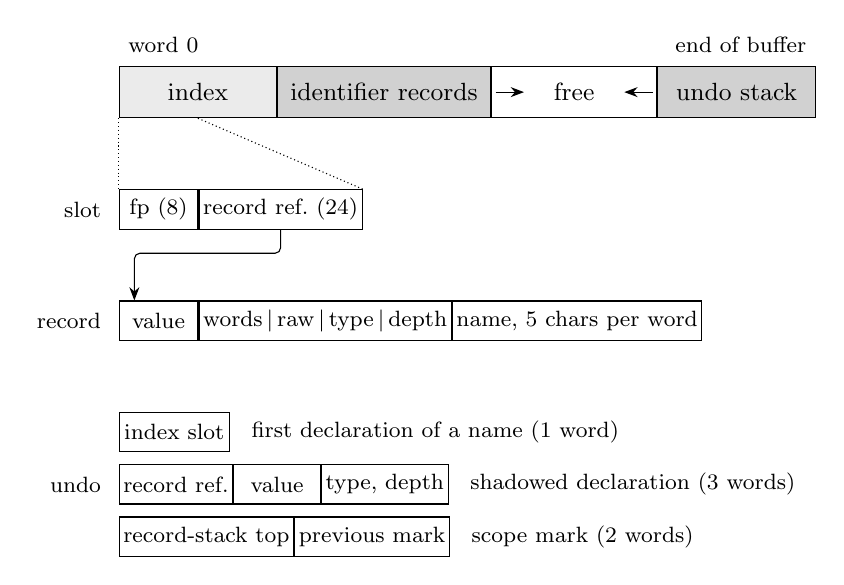
\begin{tikzpicture}[font=\small, >=Stealth,
  box/.style={draw, minimum height=6.5mm, inner sep=1.5pt, align=center},
  cell/.style={draw, minimum height=5mm, inner sep=1.5pt, align=center, font=\footnotesize}]
% the buffer
\node[box, minimum width=20mm, fill=black!8] (idx) at (0,0) {index};
\node[box, minimum width=27mm, right=0pt of idx, fill=black!18] (ids) {identifier records};
\node[box, minimum width=21mm, right=0pt of ids] (free) {free};
\node[box, minimum width=20mm, right=0pt of free, fill=black!18] (undo) {undo stack};
\draw[->] ([xshift=0.6mm]free.west) -- ++(3.6mm,0);
\draw[->] ([xshift=-0.6mm]free.east) -- ++(-3.6mm,0);
\node[above=0.5mm of idx.north west, anchor=south west, font=\footnotesize] {word 0};
\node[above=0.5mm of undo.north east, anchor=south east, font=\footnotesize] {end of buffer};
% index slot
\node[cell, minimum width=10mm, below=9mm of idx.south west, anchor=north west] (fp) {fp (8)};
\node[cell, minimum width=17mm, right=0pt of fp] (ref) {record ref.\ (24)};
\node[left=1mm of fp, font=\footnotesize, anchor=east] {slot};
\draw[densely dotted] (idx.south west) -- (fp.north west);
\draw[densely dotted] (idx.south) -- (ref.north east);
% identifier record
\node[cell, minimum width=10mm, below=9mm of fp.south west, anchor=north west] (val) {value};
\node[cell, minimum width=30mm, right=0pt of val] (meta) {words\,$|$\,raw\,$|$\,type\,$|$\,depth};
\node[cell, minimum width=27mm, right=0pt of meta] (name) {name, 5 chars per word};
\node[left=1mm of val, font=\footnotesize, anchor=east] {record};
\draw[->, rounded corners=2pt] (ref.south) -- ++(0,-3mm) -| ([xshift=2mm]val.north west);
% undo entries
\node[cell, minimum width=14mm, below=9mm of val.south west, anchor=north west] (u1) {index slot};
\node[right=1.5mm of u1, font=\footnotesize, anchor=west] (u1t) {first declaration of a name (1 word)};
\node[cell, minimum width=14mm, below=1.5mm of u1.south west, anchor=north west] (u2a) {record ref.};
\node[cell, minimum width=11mm, right=0pt of u2a] (u2b) {value};
\node[cell, minimum width=16mm, right=0pt of u2b] (u2c) {type, depth};
\node[right=1.5mm of u2c, font=\footnotesize, anchor=west] {shadowed declaration (3 words)};
\node[cell, minimum width=22mm, below=1.5mm of u2a.south west, anchor=north west] (u3a) {record-stack top};
\node[cell, minimum width=19mm, right=0pt of u3a] (u3b) {previous mark};
\node[right=1.5mm of u3b, font=\footnotesize, anchor=west] {scope mark (2 words)};
\node[left=1mm of u2a, font=\footnotesize, anchor=east] {undo};
\end{tikzpicture}
\end{document}
